\subsection{Motivational example}

In this section, we first provide a motivational example showing that the integration of a CPU into a system can introduce new timing channels that were not present in isolation.
We then discuss and formalize reentrant information flows.
Finally, we introduce platform integration contracts to capture these reentrant flows.

\begin{figure}[t]
    \begin{center}
    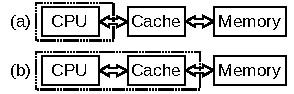
\includegraphics[width=0.6\columnwidth]{figures/verifscopecache/verifscopecache.pdf}
    \end{center}
    \vspace*{-1em}
    \caption{\label{fig:verifscopecache}
        Example verification scopes, represented as dotted boxes. (a: cache excluded) the cache is considered part of the platform. (b: cache included) the cache is considered part of the CPU.
    }
    \vspace*{-1em}
\end{figure}


\para{Methodology (cache excluded)}
Figure~\ref{fig:verifscopecache} (a) illustrates a small system in which a CPU is integrated in a platform that includes a cache and memory.
We instantiate this system, using the Kronos CPU as a case study, and a direct-mapped cache.
We use the state-of-the-art VeloCT~\cite{dinesh2025h} tool to perform constant-time verification of the CPU, which is delimited by the dotted box.
This tool verifies if only instructions of a given "safe instruction set" are executed, then the CPU runtime is independent of their operands.
We consider memory instructions as part of the safe instruction set that should execute in constant-time, in addition to arithmetic RISC-V instructions such as \texttt{add}, \texttt{sub}, \texttt{xor}, etc.

\para{Results (cache excluded)}
The Kronos verification with VeloCT, which indicates that in isolation, the CPU is constant-time secure.
In particular, this result suggests that the timing of any program made of arithmetic and memory instructions does not depend on the data that is processed, even if this data is used as memory addresses.

\para{Methodology (cache included)}
Figure~\ref{fig:verifscopecache} (b) illustrates a scenario similar to Figure~\ref{fig:verifscopecache} (a), but with the cache included in the verification scope, i.e., considered part of the CPU under verification.
Except for this point, we use the same methodology as in the previous cache excluded case.

\para{Results (cache included)}
The Kronos verification with VeloCT, which indicates that this time, the CPU is not constant-time secure.
In particular, this result implies that the program execution timing can depend on secret information used as addresses of memory instructions.

\para{Take-aways}
These results underline that while constant-time verification techniques typically operate at the level of a CPU in isolation (the platform's RTL might not yet be finalized at the CPU verification time), they may not account for all the potential interactions with other components in the system, such as caches or memory.
Therefore, the integration of the CPU into a larger system can introduce new timing channels that were not present in isolation and that are not discovered by existing constant-time verification techniques.

\subsection{Reentrant flows}

We now describe and formalize reentrant information flows, which are at the core of the timing channels that can be introduced by platform integration.

\para{Netlist graphs}
We describe a digital hardware system (e.g., the one illustrated in Figure~\ref{fig:verifscopecache}), as a netlist $G = (V, E)$, where $V$ is the set of vertices representing logic gates such as AND, OR, NOT, flip-flops, adders, and $E$ is the set of directed wires between these vertices.
We denote the subgraph of $G$ that corresponds to the CPU that is integrated in this system as $G_C = (V_C, E_C)$, where $V_C \subseteq V$ and $E_C \subseteq E$.
In particular, for all edges $(u, v) \in E_C$, both $u$ and $v$ are vertices in $V_C$.
We denote the complementary subgraph as $G_{P} = (V_{P}, E_{P})$, where $V_{P} = V \setminus V_C$ and $E_{P} = E \setminus E_C$, corresponding to the platform except the CPU that it integrates.

\para{Constant-time programs \& secret data}
For a given constant-time verification technique, let us denote by $\mathcal{P}$ the set of constant-time programs that are considered for verification.
The elements of the set $\mathcal{P}$ are triples $\tau = (P, M_p, M_s)$, where $P$ is a constant-time program, $M_p$ is the set of public memory valuations, and $M_s$ is the set of secret values that the program may depend on.
Specifically, this set $\mathcal{P}$ depends on the specific constant-time verification technique being used.
For example, for ConjunCT~\cite{dinesh2024conjunct} and VeloCT~\cite{dinesh2025h}, a triple ($P$, $M_p$, $M_s$) is considered constant-time (i.e., part of $\mathcal{P}$) if it contains no so-called "unsafe" instructions, i.e., instructions that can create an operand-dependent timing channel.
For Tan et al.~\cite{tan2025contractshadowlogic}, a triple ($P$, $M_p$, $M_s$) is considered constant-time (i.e., part of $\mathcal{P}$) if it ensures that the program's control flow and all memory accesses are independent of secret data.
The conditions for a program to be constant-time with respect to ConjunCT's and VeloCT's definition are stricter than those of Tan et al.~\cite{tan2025contractshadowlogic}, as the latter generally forbid branches, for instance.
Inclusively more restrictive constraints imply an inclusively smaller set $\mathcal{P}$ of constant-time programs.

\para{Secret propagation}
Constant-time verification techniques generally proceed by analyzing whether the valuation of a state element that captures timing differences can be influenced by secret information.
For example, Tan et al.~\cite{tan2025contractshadowlogic}, LeaVe~\cite{wang2023specification}, ConjunCT~\cite{dinesh2024conjunct} and VeloCT~\cite{dinesh2025h} monitor whether secret information can influence the commit signal, while \ucfi~\cite{ceesay2024mucfi} monitors whether secret information can influence a microarchitectural program counter structure.

We define the \emph{valuation sequence} $\nu$ of a vertex.
For a vertex $v \in V$ and a triple $\tau = (P, M_p, M_s)$, the valuation sequence $\nu_\tau(v)$ is the clock-accurate infinite sequence of valuations that the vertex takes during the execution of a program $P$ with respect to the memory valuations $M_p$ and $M_s$, starting from the CPU's and platform's reset state, assumed deterministic.
Note that we assume determinism for simplicity without loss of generality; to account for non-determinism, we could consider a set $\nu_\tau^{\text{non-det}}(v)$ of all possible valuation sequences instead of a single sequence $\nu_\tau(v)$, without change in the following reasoning.

We denote by $V^s$ the set of vertices in $V$ whose valuation sequence can be influenced by secret information when the system executes a program written in constant-time with respect to the secret data.
An element $v \in V$ belongs to $V^s$ if and only if there exist two triples $\tau = (P, M_p, M_s)$ and $\tau' = (P, M_p, M_s')$ that only differ in $M_s'$, and such that $\tau \in \mathcal{P}$ and $\tau' \in \mathcal{P}$ but $\nu_\tau(v) \neq \nu_{\tau'}(v)$.
We say that a vertex $v \in V$ is \emph{secret-dependent} if it belongs to $V^s$.

For a secret-dependent vertex $v \in V^s$, we define the set $P^s_v$ of \emph{secret propagation paths} to be the paths in the graph $G$ that connect the source of secrets (that can take the value $M_s$ or $M_s'$) to $v$, where all the vertices in the path are secret-dependent.
In particular, $P^s_v$ is non-empty.
Indeed, if $v \in V^s$, then at least one predecessor $u \in V$ of $v$ must also be secret-dependent, which recursively constructs a path in $P^s_u$.

Let us consider a strict subgraph $G' = (V', E') \subsetneq G$ and a vertex $v \in V'^s$.
A path $p$ in $P^s_v$ is said to be \emph{reentrant} in $G'$ if it contains at least one vertex $u \in V \setminus V'$, i.e., a vertex that is outside of $G'$.
Note that this $u$ also belongs to $V^s\setminus V'$ because all nodes in $p$ are secret-dependent by definition of $P^s_v$.
If all paths in $P^s_v$ are reentrant in $G'$, then we say that the vertex $v$ is \emph{fully reentrant} in $G'$.

\para{Example}
Let us consider again the system Figure~\ref{fig:verifscopecache} (a) where $\mathcal{P}$ describes programs where secret data, which is for example initially stored in a well-specified general-purpose register, can be used as the address of a memory instruction.
Because the CPU itself does not contain caches or other components whose timing depends on memory addresses, for $v$ designating the commit signal (for LeaVe~\cite{wang2023specification}, Tan et al.~\cite{tan2025contractshadowlogic}, ConjunCT~\cite{dinesh2024conjunct} or VeloCT~\cite{dinesh2025h}), or a microarchitectural PC signal (\ucfi~\cite{ceesay2024mucfi}), $v$ is fully-reentrant in the CPU, if we consider $G$ being the whole platform, and $G'$ being the CPU.

\subsection{Contracts}

The key idea of our work is to define \emph{platform timing contracts} that capture the possible reentrant information flows in the CPU that are allowed by a given platform.
Since the interface between the output signals of a CPU and the rest of a SoC is usually much simpler than the hardware-software interface, these contracts are expected to be simpler than existing hardware-software contracts.

\para{Interface}
We base our analysis on the widely-studied RISC-V ISA.
The output signals of a RISC-V CPU are all through memory interfaces, which are made of data and control signals.
% \fls{TODO Maybe change all "CPU"'s with "CPU core"}
Data signals transport the data to be read or written to or from the memory.
Control signals transport the information about the memory transaction, such as the memory address, handshake signals, and depending on the memory bus protocol (e.g., AMBA AXI~\cite{arm_amba} or TileLink~\cite{tilelink_spec}), further control signals such as the type of transaction and the size of the data to be read or written.
Input signals of a RISC-V CPU can be more diverse, including memory input data and control signals, interrupt lines, and various other control signals such as clock gating signals.

\para{Platform timing contracts}
Platform timing contracts aim to ensure that state elements that capture timing differences (e.g., a commit signal or a microarchitectural program counter) \emph{are not fully reentrant} in the CPU.
To ensure this, a platform timing contract specifies an upper bound of the information flows between the output signals of the CPU and its input signals.
We express a platform timing contract as a list of rules, listed per CPU output signal.
% In Section~\ref{sec:instrumentation}, we introduce synthesizable constructs that create paths between secret sources and sinks, to ensure that the sets $P^s_v$ are not empty for these sinks, preventing these sinks from being fully-reentrant.
% \textcolor{red}{TODO Continuer ici.}


\para{Example contracts}
Fig.~\ref{fig:contract_equations} provides four example contracts for a RISC-V CPU with a Von Neumann architecture.
We model the memory interface as an outbound address bus (\texttt{addr}), an inbound and an outbound memory data port (respectively \texttt{rdata} and \texttt{wdata}), and a simple valid-ready handshake protocol (inbound \texttt{resp} and outbound \texttt{req}), similar to the \texttt{req} and \texttt{gnt} handshake signals in the Hardware Processing Engines (HWPE) 2.0 interface protocol~\cite{pulpHWPEMem}.
Fig.~\ref{fig:contract_equations}'s contract C1 defines a simple integration contract for a platform with ideal memory that responds with a constant timing (i.e., that is address-independent).
A change in the memory transaction control signals from the CPU can only change the returned value.
Only the request signal (\texttt{req}) can affect the existence, and hence the timing, of a memory response.
% Indeed, a change in the address of a read, for example, might read from a memory cell that contains a different value, and a change, for example in the timing of some request signal will affect the timing of the memory response, and hence the memory read data at some point in time.
The diamond $\lozenge$ underlines that the right-hand side of the implication can happen at any time and for any number of times after the left-hand side.
% \fls{Maybe I should explain more intuitions like why req and addr actually have exactly the same effect.}
Contract C2 adds timing dependence on the memory address, which is typical of structures like caches.
In this contract, \texttt{req} and \texttt{addr} have an identical clause. Indeed, a change in the address of a read, for example, can change a cache miss into a cache hit, changing the timing of the response, and hence its value at some point in time, including the \texttt{gmt} control signal and the \texttt{rdata} data signals.
Contract C3 models data-dependent interrupts (\texttt{int}) and timing.
That is, the \emph{reentrant secret propagation paths} (see Section~\ref{sec:reentrant}) all go through a specific set of memory addresses only.
For example, some peripheral might be controlled through memory-mapped registers such as an interrupt controller~\cite{riscv_plic_spec_1_0_0}.

\para{Conditional refinements}
\fls{TODO ensure to reference section III.B.}
Contract C3 implies that writing tainted, i.e., secret, data to memory with a specific address that is not tainted might always trigger an interrupt or affect the timing of the memory response.
\fls{TODO Fix this sentence.}
In some settings, this might be true only for specific address ranges where peripherals are mapped, but parts of the memory address range can typically be used in a data-independent timing.
\fls{Be more concrete here.}
To refine this contract, we introduce address-dependent contracts as in Contract C4, where the right-hand side of the implication depends on the memory address set \texttt{periph\_range}, which is a fixed set of addresses.
% Note that the contract could also be refined by making the interrupts dependent on the written data.
% For example, an interrupt might never be triggered, whatever the address, if the written data is zero, for the class of platforms of interest for the CPU integrator.
% In verification, such constraints can be expressed as data-independent timing assuming that the CPU does not write to memory addresses in \texttt{periph\_range} with tainted data.
For example, this can be achieved with RISC-V Physical Memory Protection (PMP) in a setting where the most privileged execution mode does not access secret data and protects the \texttt{periph\_range} address range from being accessed from lower privileges, in the philosophy of trusted execution environments~\cite{lee2019keystone,costan2016sanctum,arm2009trustzone,mcgillion2015opentee,schneider2022sok,bourgeat2018mi6,brasser2022tcx}.

% \fls{TODO Say that we will have a reference contract later for the end-to-end attack.}
% \fls{TODO Say the right-hand side can be anytime after, and for any number of time. Maybe write this as an LTL formula.}


\begin{figure}
    \begin{center}
    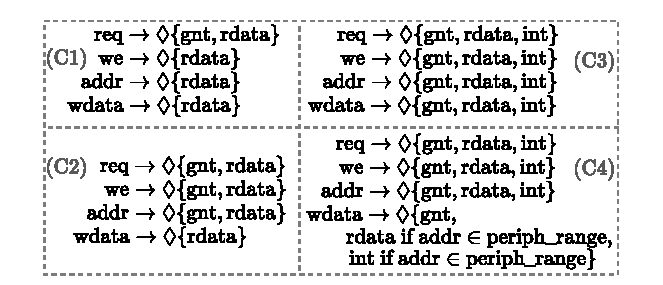
\includegraphics[width=\columnwidth]{figures/contract_equations/contract_equations.pdf}
    \end{center}
    \vspace{-1.8em}
    \caption{Example platform contracts.}
    \label{fig:contract_equations}
    \vspace*{-1.5em} 
\end{figure}

% \begin{equation}
% \label{dict:contract_nocache}
% \begin{array}{rcl}
% \text{req} & \rightarrow & \lozenge \{ \text{gnt}, \text{rdata}\} \\
% \text{we} & \rightarrow & \lozenge \{\text{rdata}\} \\
% \text{addr} & \rightarrow & \lozenge \{ \text{rdata}\} \\
% \text{wdata} & \rightarrow & \lozenge \{ \text{rdata} \} \\
% \end{array}
% \end{equation}

% \begin{equation}
% \label{dict:contract_cache_nointerrupt}
% \begin{array}{rcl}
% \text{req} & \rightarrow & \lozenge \{ \text{gnt}, \text{rdata}\} \\
% \text{we} & \rightarrow & \lozenge \{ \text{gnt}, \text{rdata}\} \\
% \text{addr} & \rightarrow & \lozenge \{ \text{gnt}, \text{rdata}\} \\
% \text{wdata} & \rightarrow & \lozenge \{ \text{rdata} \} \\
% \end{array}
% \end{equation}

% \begin{equation}
% \label{dict:contract_cache_interrupt}
% \begin{array}{rcl}
% \text{req} & \rightarrow & \lozenge \{ \text{gnt}, \text{rdata}, \text{interrupt}\} \\
% \text{we} & \rightarrow & \lozenge \{ \text{gnt}, \text{rdata}, \text{interrupt}\} \\
% \text{addr} & \rightarrow & \lozenge \{ \text{gnt}, \text{rdata}, \text{interrupt}\} \\
% \text{wdata} & \rightarrow & \lozenge \{ \text{gnt}, \text{rdata}, \text{interrupt} \} \\
% \end{array}
% \end{equation}

% \begin{equation}
% \label{dict:contract_cache_interrupt_addressdependent}
% \begin{array}{rcl}
% \text{req}  & \rightarrow & \lozenge \{ \text{gnt}, \text{rdata}, \text{interrupt}\} \\
% \text{we}  & \rightarrow & \lozenge \{ \text{gnt}, \text{rdata}, \text{interrupt}\} \\
% \text{addr} & \rightarrow & \lozenge \{ \text{gnt}, \text{rdata}, \text{interrupt}\} \\
% % \text{wdata} & \rightarrow & \lozenge \{ \text{rdata}, \text{interrupt} \} \\
% \text{wdata} & \rightarrow & \lozenge \{ \text{rdata}, \\
% & & \text{gnt if addr in periph\_range} \\
% & & \text{interrupt if addr in periph\_range} \} \\

% \end{array}
% \end{equation}

\para{Ordering of \pics}
Like for sinks, we can define a partial ordering of \pics.
We say that a contract A is (inclusively) stronger than a contract B if for every output of the CPU (i.e., the left-hand side of the arrow in the contract), the set of possible CPU inputs tainted by this output in contract A is a subset of the set of possible CPU inputs tainted by this output in contract B.
Said otherwise, contract A is stronger than contract B if it allows for fewer possible information flows.
For example, Contract C4 is stronger than Contract C3, and Contract C2 is stronger than Contract C3.
A CPU that is verified to have a constant-time behavior with respect to a stronger \pic is also verified with respect to a weaker \pic.

\begin{figure}
    \begin{center}
    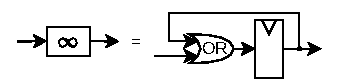
\includegraphics[width=.7\columnwidth]{figures/stickyone/stickyone.pdf}
    \end{center}
    \vspace*{-1em}
    \caption{Sticky-one operator. The sticky-one is reset to zero (not illustrated in the figure) and sticks to 1 once it is set.}
    \label{fig:stickyone}
    \vspace*{-.4em}
\end{figure}


\begin{figure}[t]
    \begin{center}
    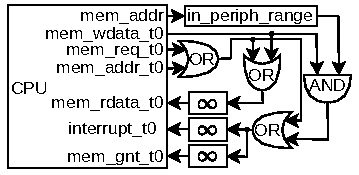
\includegraphics[width=.7\columnwidth]{figures/picinstrum_taints/picinstrum_taints.pdf}
    \end{center}
    \vspace*{-1em}
    \caption{\Pici for a design whose information flows are tracked with dynamic information flow tracking instrumentation. Signals that end with \texttt{t0} represent the taint signals~\cite{tiwari2009complete,solt2022cellift}.
    }
    \label{fig:pic_instrum_taints}
    \vspace*{-.4em}
\end{figure}

\begin{figure}[t]
    \begin{center}
    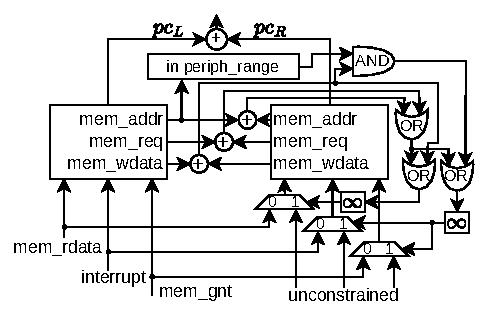
\includegraphics[width=0.9\columnwidth]{figures/picinstrum_miter/picinstrum_miter.pdf}
    \end{center}
    \vspace*{-1em}
    \caption{\Pici for a design whose information flows are tracked with a miter. }
    \label{fig:pic_instrum_miter}
    \vspace*{-.4em}
\end{figure}
